\documentclass[a4paper]{article}

\usepackage[english]{babel}
\usepackage[utf8]{inputenc}
\usepackage{amsmath}
\usepackage{graphicx}
\usepackage[colorinlistoftodos]{todonotes}
\usepackage[T1]{fontenc}	%ADDED for << og >>
\usepackage{enumitem}		%ADDED for smaller spacing


\title{Assinment43}

\author{pebj, smot}

\date{\today}

\begin{document}
\maketitle

\section{Most appropriate component tests}
	We have chocen to make a component test of all our  subsystems facadas, this inclode EventLogic, Season and AccountLogic. We are also component testing EventComponet becourse it is isentiel for transporting data in our system. We have chocen not to make stubs for EventComponent, Account og Notification, becourse to make the stubs work right, we would have to implement almost the same code as the original. Given that the classes are all data classes, we see nothing wrong with it.
    
\section{Integration test strategy}
   	The strategy we are using is one of the Horizontal integration testing strategies, the bottom-up strategy. 
    	Becourse we dit not have enough time to develop to many test-stubs


	\begin{table}
		\centering
		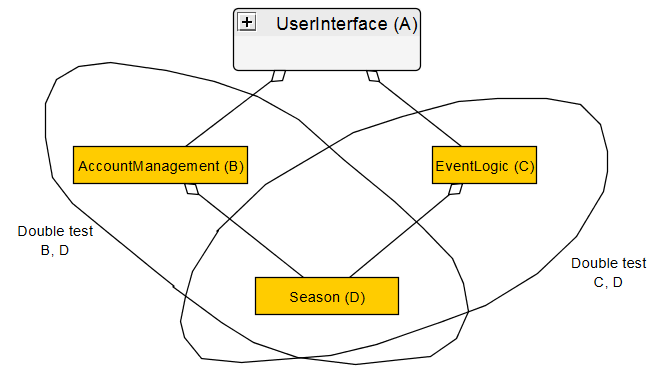
\includegraphics[width=1\textwidth]{UMLtestDiagram.PNG}\\
		\caption{Bottom-up test strategy. After unit testing subsystems A, B, C and D, the bottom up integration 
			test proceeds with the double tests B-D and C-D.}
	\end{table}


\end{document}